% VulnHunterX — arXiv-ready LaTeX source
% Compiled with: pdflatex vulnhunterx.tex (twice for cross-references)
% No external bibliography file: references are inline in thebibliography.

\documentclass[11pt,a4paper]{article}

% ---------- Packages ----------
\usepackage[utf8]{inputenc}
\usepackage[T1]{fontenc}
\usepackage{lmodern}
\usepackage[margin=1in]{geometry}
\usepackage{microtype}
\usepackage{amsmath}
\usepackage{amssymb}
\usepackage{graphicx}
\usepackage{xcolor}
\usepackage{booktabs}
\usepackage{array}
\usepackage{longtable}
\usepackage{tabularx}
\usepackage{enumitem}
\usepackage{listings}
\usepackage{textcomp}
\usepackage{url}
\usepackage[colorlinks=true,linkcolor=NavyBlue,citecolor=NavyBlue,urlcolor=NavyBlue]{hyperref}
\usepackage[svgnames]{xcolor}

% ---------- Listings styles ----------
\definecolor{codebg}{rgb}{0.97,0.97,0.97}
\definecolor{codeframe}{rgb}{0.85,0.85,0.85}
\definecolor{codecomment}{rgb}{0.35,0.55,0.35}
\definecolor{codekey}{rgb}{0.00,0.20,0.55}
\definecolor{codestr}{rgb}{0.60,0.10,0.10}

\lstdefinestyle{vhxbase}{
  basicstyle=\ttfamily\footnotesize,
  backgroundcolor=\color{codebg},
  frame=single,
  rulecolor=\color{codeframe},
  framesep=4pt,
  xleftmargin=6pt,
  xrightmargin=6pt,
  columns=fullflexible,
  keepspaces=true,
  breaklines=true,
  breakatwhitespace=false,
  showstringspaces=false,
  upquote=true,
  tabsize=2,
  literate=%
    {→}{{$\rightarrow$}}1
    {←}{{$\leftarrow$}}1
    {≥}{{$\geq$}}1
    {≤}{{$\leq$}}1
    {≈}{{$\approx$}}1
    {…}{{\ldots}}1
    {×}{{$\times$}}1
    {·}{{$\cdot$}}1
    {∈}{{$\in$}}1
    {–}{{--}}1
    {—}{{---}}1
    {§}{{\S}}1,
}

\lstdefinelanguage{yamlex}{
  keywords={true,false,null,True,False,None},
  keywordstyle=\color{codekey}\bfseries,
  comment=[l]{\#},
  commentstyle=\color{codecomment}\itshape,
  morestring=[b]',
  morestring=[b]",
  stringstyle=\color{codestr},
  sensitive=true,
}

\lstdefinelanguage{jsonex}{
  morestring=[b]",
  stringstyle=\color{codestr},
  literate=%
    *{0}{{{\color{codekey}0}}}{1}
     {1}{{{\color{codekey}1}}}{1}
     {2}{{{\color{codekey}2}}}{1}
     {3}{{{\color{codekey}3}}}{1}
     {4}{{{\color{codekey}4}}}{1}
     {5}{{{\color{codekey}5}}}{1}
     {6}{{{\color{codekey}6}}}{1}
     {7}{{{\color{codekey}7}}}{1}
     {8}{{{\color{codekey}8}}}{1}
     {9}{{{\color{codekey}9}}}{1}
     {:}{{{\color{black}{:}}}}{1}
     {,}{{{\color{black}{,}}}}{1}
     {\{}{{{\color{black}{\{}}}}{1}
     {\}}{{{\color{black}{\}}}}}{1}
     {[}{{{\color{black}{[}}}}{1}
     {]}{{{\color{black}{]}}}}{1},
}

\lstdefinelanguage{bashex}{
  morecomment=[l]{\#},
  commentstyle=\color{codecomment}\itshape,
  morestring=[b]',
  morestring=[b]",
  stringstyle=\color{codestr},
  keywords={cd,ls,mkdir,rm,cp,mv,grep,git,echo,export,if,then,else,fi,for,do,done,while,uv,pip,python,npx},
  keywordstyle=\color{codekey}\bfseries,
}

\lstset{style=vhxbase}

% ---------- Title ----------
\title{
\textbf{VulnHunterX}: \\
Guided-Question Multi-Turn LLM Verification \\
for Cost-Efficient SAST False-Positive Reduction
}

\author{
thientc \\
VinSOC Cyber \\
\texttt{v.thientc6@vinsoc.vn}
}

\date{}

% ---------- Body ----------
\begin{document}

\maketitle

\begin{abstract}
\noindent
Static application security testing (SAST) tools such as CodeQL,
Semgrep, OpenGrep, and SonarQube are now standard in secure software
development life-cycles, yet their over-approximating analyses generate
false-positive (FP) rates of 30--80\% in production. The dominant
industrial cost of SAST is therefore not analysis time but
\textbf{expert triage time}. Recent work has explored Large Language
Models (LLMs) as an automated triage layer, with the highest-accuracy
results requiring frontier models (GPT-4-class) at a cost prohibitive
at the scale of real codebases ($\approx$US\$2{,}758 to triage
7{,}194 warnings, per LLM4FPM, 2024). Frontier-model security reasoning
is also brittle: SecLLMHolmes (IEEE S\&P 2024) reports state-of-the-art
LLMs at $\approx$40\% accuracy on hand-crafted security scenarios,
attributing the failure to \emph{pattern-matching without anchoring to
specific code evidence}.

Reasoning structure, not model size, moves the cost-vs-accuracy
frontier. This paper presents \textbf{VulnHunterX}, an open-source
framework that operationalizes the \emph{Vulnhalla methodology}: a
verification pipeline driven by \textbf{guided questions} that
decompose expert triage into atomic, evidence-bound sub-tasks. Four
primitives carry the framework. Per-rule \textbf{guided question banks}
force the model to anchor each verdict in declarations, sizes,
free-sites, alias sets, and control-flow paths, and close with a
\emph{decision rule} that turns the verdict into a derivable theorem.
An \textbf{answer-before-verdict protocol} requires the LLM to answer
every guided question and emit an explicit data-flow trace before the
verdict field is generated, so autoregressive conditioning ties the
verdict to stated evidence. A \textbf{context broker} with a fixed
context-request vocabulary, backed by a tree-sitter fallback covering
seven languages, supports cheap multi-turn refinement without
re-running the underlying SAST engine and keeps the protocol working
on repositories whose CodeQL database cannot be built. An
\textbf{extensible architecture} makes SARIF the sole contract between
SAST engines and the verification core: 73 custom CodeQL queries and
47 custom Semgrep / OpenGrep rules layer onto built-in suites through
a single profile flag, custom findings route through the same
guided-question matcher built-in rules use, and an audit script gates
the routing wiring in CI.

The framework, six guided-question corpora (C/C++, Java, JavaScript,
PHP, Python, Go; 4{,}676 total lines / 342 per-rule templates), the
73 custom CodeQL queries and 47 custom Semgrep / OpenGrep rules, the
rule-coverage audit script, and the benchmark harness are released
under the MIT license. Comparative empirical evaluation against
frontier-model and local-model baselines on Juliet C/C++, OWASP
Benchmark (Java), and CASTLE is reserved for a companion paper.
\end{abstract}

\medskip
\noindent\textbf{Keywords:} static analysis, false positive reduction,
large language models, guided questions, multi-turn verification,
CodeQL, Semgrep, custom rules, developer extensibility, secure software
engineering.

% =====================================================================
\section{Introduction}
\label{sec:intro}

Software vulnerabilities continue to dominate cybersecurity incident
reports; the MITRE Top-25 list and the Verizon DBIR consistently
attribute a majority of breaches to memory-safety, injection, and
access-control flaws that \textbf{static analysis can, in principle,
detect}. CodeQL, Semgrep, OpenGrep, SonarQube, Coverity, and similar
tools encode such vulnerability classes as data-flow or pattern queries
over a relational or graph representation of source code. Their
analyses are deliberately \textbf{over-approximating}: they flag every
program point that \emph{might} be vulnerable, and consequently produce
a substantial fraction of false positives.

The empirical FP rate of modern SAST tools varies by rule and codebase
but is consistently in the 30--80\% range (Christakis \& Bird, ASE
2016; Johnson et al., FSE 2013; Imtiaz et al., 2019). The
industrial response is a \textbf{manual triage} stage in which a
security engineer reviews each alert. At the scale of a contemporary
monorepo this is the single largest cost item in a SAST programme; it
is also a documented source of analyst fatigue and inconsistent
dispositions.

\subsection{Problem statement}

Let $F = \{f_1, \ldots, f_n\}$ be the set of findings emitted by one or
more SAST tools on a codebase $C$. Each $f_i$ is a tuple
$(\textit{rule\_id}, \textit{location}, \textit{message},
\textit{metadata})$. Let
$V^{*}\!:\!F\!\to\!\{\textsc{tp},\textsc{fp}\}$ be the ground-truth
oracle (a sufficiently expert human reviewer with unbounded budget).
The \emph{triage problem} is to construct an automated function
$V\!:\!F\!\to\!\{\textsc{tp},\textsc{fp},\textsc{nmd}\}$ (where
\textsc{nmd} denotes ``Needs More Data'' and triggers human review)
that maximizes precision and recall against $V^{*}$ while minimizing
monetary cost and human-review volume.

The literature has explored two principal automation strategies for
$V$: classical machine-learning classifiers over alert features
(Heckman \& Williams, 2011; Yoon et al., 2014) and, more recently,
LLM-based triage (LLM4FPM, 2024; ZeroFalse, 2025; LLMxCPG,
USENIX Security 2025). LLM-based approaches dominate the recent
literature because they generalize across rules and codebases without
re-training, but they introduce two new challenges that this paper
directly addresses:

\begin{itemize}[leftmargin=*]
\item \textbf{C1. Reasoning grounding.} Free-form LLM verdicts
  hallucinate; pattern-matched convictions are common, especially on
  synthetic benchmarks containing adjacent positive and negative
  variants (Juliet's bad/good pairs).
\item \textbf{C2. Cost.} At frontier-model list pricing, full-coverage
  triage of a production-scale alert stream is economically infeasible.
\end{itemize}

A third challenge is engineering rather than scientific but blocks
deployment in practice:

\begin{itemize}[leftmargin=*]
\item \textbf{C3. Tool, language, and signature heterogeneity.} Real
  SAST programmes run multiple engines (CodeQL + Semgrep + OpenGrep +
  SonarQube) over multiple languages, and individual defenders carry
  threat models that built-in rule suites do not cover --- proprietary
  RPC frameworks, internal serialization formats, domain-specific
  dangerous APIs. Existing LLM-triage systems are typically wired to a
  single engine, a single language, and a fixed rule set, making both
  engine-switching and rule-extension costly.
\end{itemize}

\subsection{Research questions}

This paper investigates four research questions:

\begin{itemize}[leftmargin=*]
\item \textbf{RQ1 (Reasoning grounding).} Can a structured
  \emph{guided-question} protocol that forces evidence-anchored answers
  before verdict generation materially reduce LLM hallucination on SAST
  triage, relative to free-form prompting?
\item \textbf{RQ2 (Extensibility).} Can the protocol generalize across
  multiple SAST engines, multiple source languages, \emph{and}
  developer-authored custom signatures, without changing the
  verification core?
\item \textbf{RQ3 (Context broker).} Does a fixed-vocabulary context
  broker support cheap multi-turn refinement without sacrificing the
  precision a free-form context-retrieval channel would offer, and
  how should it degrade when the primary (CodeQL-derived) backend is
  unavailable?
\item \textbf{RQ4 (Cross-language transferability).} To what extent do
  guided-question templates authored for one language transfer to
  semantically similar languages, and how much of the per-rule corpus
  is language-universal as opposed to language-specific?
\end{itemize}

This paper is a methodological contribution; comparative empirical
validation of RQ1 against baselines on Juliet C/C++, OWASP Benchmark
(Java), and CASTLE is reserved for a companion evaluation paper. RQ2
and RQ4 are answered constructively in
Section~\ref{sec:architecture}, which exhibits the extensibility
contract across three engines, six languages, and 120 shipped custom
signatures. RQ3 is answered constructively in Section~\ref{sec:broker}
(broker design plus tree-sitter fallback), with quantitative
validation of the cost-precision trade-off also reserved for the
companion paper.

\subsection{Contributions}
\label{sec:contributions}

\begin{itemize}[leftmargin=*]
\item \textbf{Guided-question methodology with an answer-before-verdict
  protocol} (Sections~\ref{sec:questions}--\ref{sec:protocol}) that
  operationalizes cognitive-task-analysed expert triage as a per-rule
  checklist of evidence-seeking questions terminated by a decision
  rule. The response schema positions answers and the data-flow trace
  before the verdict token, so autoregressive conditioning makes the
  verdict a function of stated evidence rather than free judgment.
\item \textbf{Context broker with a tree-sitter fallback}
  (Section~\ref{sec:broker}) over a fixed-vocabulary request grammar.
  The fixed vocabulary makes multi-turn conversation cheap (no live
  SAST re-runs) and rejects requests outside the grammar instead of
  returning plausible nonsense. When the primary CodeQL extraction
  backend fails to build a database, a seven-language tree-sitter
  extractor populates the same CSV schema, so the broker interface is
  preserved.
\item \textbf{Extensible SARIF-based architecture}
  (Section~\ref{sec:architecture}) in which SARIF is the sole contract
  between SAST engines and the verifier. The shipped release includes
  CodeQL/Semgrep/OpenGrep adapters, 73 custom CodeQL queries and 47
  custom Semgrep/OpenGrep rules layered through five named profiles,
  a rule-id matcher that routes custom and built-in findings through
  the same guided-question pipeline, and an audit script that gates
  the routing wiring in CI. Extensibility is multi-engine,
  multi-language, and multi-author at one declarative contract.
\item \textbf{Open release} (Section~\ref{sec:repro}) of the framework,
  six-language guided-question corpora, custom rule packs, the audit
  script, and the benchmark harness under MIT.
\end{itemize}

% ---- Architecture figure (overview) ----
\begin{figure}[t]
  \centering
  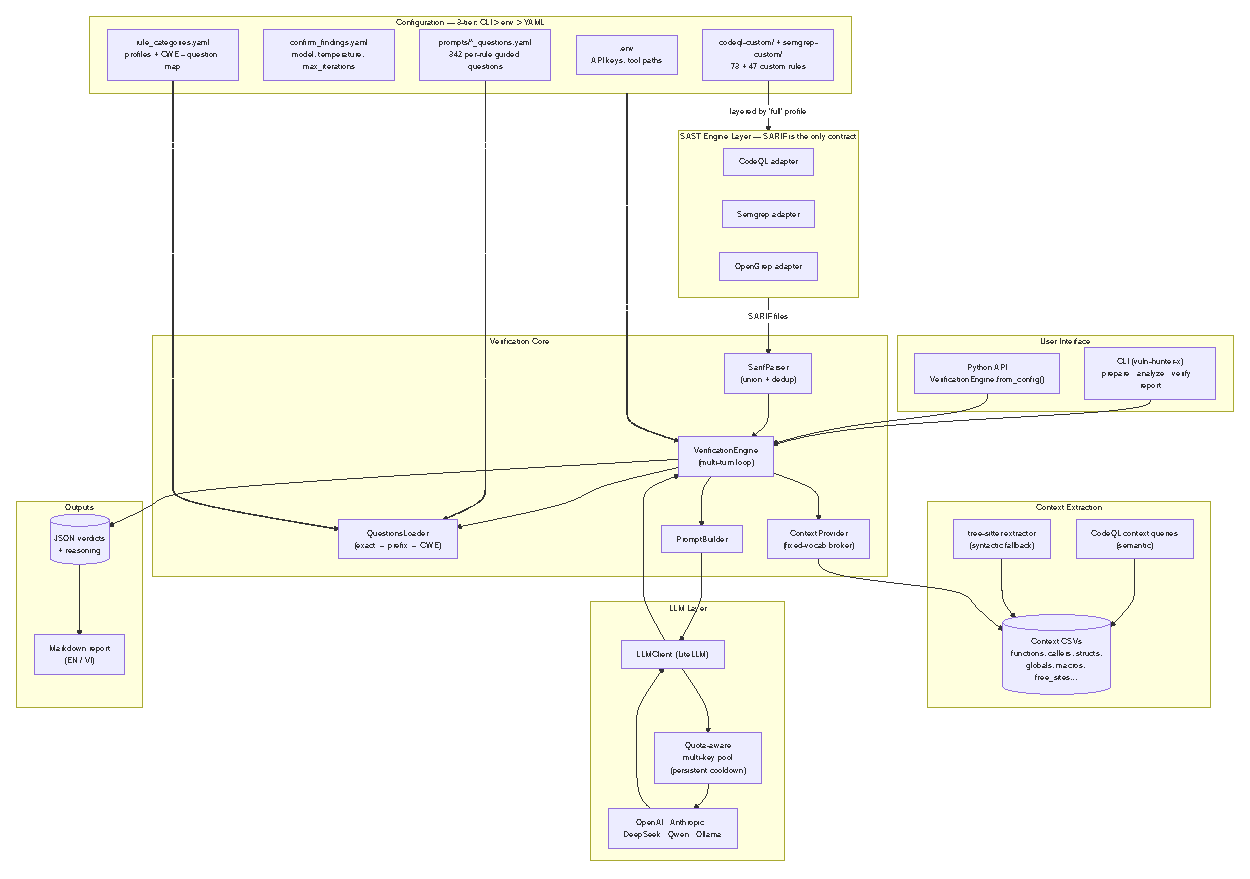
\includegraphics[width=\textwidth,height=0.55\textheight,keepaspectratio]{figures/architecture.pdf}
  \caption{VulnHunterX framework architecture. SARIF acts as the sole
  contract between SAST engine adapters (CodeQL, Semgrep, OpenGrep) and
  the verification core. Context CSVs --- extracted by CodeQL queries
  with a tree-sitter fallback --- feed the multi-turn LLM verification
  loop without re-running the underlying SAST engine.}
  \label{fig:architecture}
\end{figure}

% =====================================================================
\section{Background and Related Work}
\label{sec:related}

\subsection{Static analysis and the false-positive problem}

CodeQL (Avgustinov et al., SLE 2016) compiles source code into a
relational database and expresses vulnerability rules as Datalog-like
queries over control- and data-flow predicates. Semgrep
(returntocorp.com) uses syntactically-grounded pattern templates with
limited inter-procedural reasoning. OpenGrep is the
community-maintained open fork of Semgrep (license-aligned,
semantically equivalent for our purposes). All three emit SARIF
(OASIS, 2020), the industry-standard JSON schema for analysis results,
with structured \texttt{precision} and \texttt{security-severity}
fields encoding the rule author's a-priori confidence.

The \emph{unsoundness/incompleteness trade-off} (Rice, 1953; in
practice Cousot \& Cousot's abstract interpretation framing) means
SAST tools must choose between missing bugs (false negatives) and
over-flagging (false positives). Production rules are tuned
conservatively, accepting an FP rate that manual triage is then
expected to absorb.

\subsection{Classical FP-reduction approaches}

Earlier work used statistical learning over alert features:
Heckman and Williams (2011) survey twenty-one classifier-based systems;
Hanam et al. (2014) cluster alerts by program features; Yoon et al.
(2014) use active learning to amortize reviewer labels. These
approaches rely on historical labels and degrade across rules and
codebases.

\subsection{LLM-based triage}
\label{sec:llm-triage}

The recent LLM-based literature varies along two axes,
\textbf{prompting strategy} and \textbf{context construction},
summarized in Table~\ref{tab:positioning}.

\begin{table}[t]
\centering
\caption{Positioning of VulnHunterX against the recent LLM-based SAST
triage literature.}
\label{tab:positioning}
\footnotesize
\begin{tabularx}{\textwidth}{@{}lllXX@{}}
\toprule
\textbf{System} & \textbf{Prompting} & \textbf{Context} &
\textbf{Model class} & \textbf{Scale / scope} \\
\midrule
LLM4FPM (2024)    & Multi-turn (5)     & eCPG slices          & Qwen2.5-32B     & 7{,}194 Juliet warnings (C/C++) \\
ZeroFalse (2025)  & Zero-shot CoT      & CodeQL alert + slice & GPT-4-class     & 1{,}974 OWASP Java alerts       \\
SecLLMHolmes (2024) & Single-shot      & Hand-crafted         & GPT-4 / Claude  & 228 scenarios, 8 CWEs           \\
LLMxCPG (2025)    & Single-shot        & CPG-sliced (68--91\%)& Mixed           & Multi-CWE C/C++                  \\
CASTLE (2025)     & Benchmark only     & n/a (250 programs)   & n/a             & 25 CWEs (benchmark)             \\
\midrule
\textbf{VulnHunterX} & \textbf{Multi-turn guided-question + decision rule} & \textbf{Brokered context + slice} & \textbf{Engine-agnostic; defender-extensible} & \textbf{6 langs, 3 SAST tools, 120 custom signatures} \\
\bottomrule
\end{tabularx}
\end{table}

Three gaps motivate this work: (i) no prior system \emph{enforces}
evidence-bound reasoning at the response-schema level, (ii) prior
systems target a single SAST engine and single language family, and
(iii) prior systems treat the rule set as fixed by the engine vendor
rather than as an extension surface authored by defenders themselves.

We compare against the five most closely related systems individually:

\paragraph{LLM4FPM (Su et al., 2024).} Evaluates Qwen2.5-32B on 7{,}194
Juliet C/C++ warnings across seven memory-safety CWEs with a five-turn
dialogue and eCPG-derived slices. LLM4FPM establishes that multi-turn
local-model triage is feasible at scale and provides the per-warning
token budget ($\sim$6{,}848 tokens) that frames our cost model. Our
differences: (i) we \emph{enforce} answer-before-verdict at the JSON
schema rather than via prompt instructions only, (ii) we slice through
a CodeQL-derived CSV broker rather than an eCPG, and (iii) we ship a
per-rule guided-question corpus rather than a single generic prompt,
which we expect to widen the gap on injection-class rules where
multi-hop reasoning matters less than per-rule pattern discrimination.

\paragraph{ZeroFalse (Mohajer et al., 2025).} Zero-shot chain-of-thought
triage of 1{,}974 CodeQL alerts on the OWASP Java Benchmark.
ZeroFalse's headline finding --- that zero-shot CoT outperforms
few-shot on this benchmark --- informs the \verb|--max-iterations 1|
configuration we expose as an inline-CI mode. Where ZeroFalse uses a
single LLM call, our pipeline retains the option to escalate to
multi-turn for NMD responses; the two are complementary along the
latency/accuracy axis.

\paragraph{LLMxCPG (Risse et al., 2025).} CPG-guided slicing reduces
LLM input by 68--91\% while preserving vulnerability context, applied
as a single-shot detector across multiple CWEs. Our regex-based slicer
is an explicit Phase~1 approximation of LLMxCPG; CPG-based slicing
through CodeQL data-flow is planned as future work. Orthogonally,
LLMxCPG is a detector while VulnHunterX is a triage layer above
existing detectors.

\paragraph{SecLLMHolmes (Ullah et al., 2024).} A negative-result
benchmark demonstrating that frontier LLMs (GPT-4, Claude) cap at
$\sim$40\% accuracy on 228 hand-crafted security scenarios, attributing
failure to pattern matching without code evidence. We treat
SecLLMHolmes both as motivation (answer-before-verdict directly targets
the diagnosed failure mode) and as a planned evaluation target in the
companion empirical paper.

\paragraph{CISC (Li et al., 2025).} Confidence-weighted self-consistency
reduces the LLM samples needed for stable majority voting by 46\%. We
expose this as the optional \texttt{force\_decision\_samples} parameter
for NMD-handling; it is off by default to keep the protocol minimal.

\subsection{The Vulnhalla methodology}

Vulnhalla, developed by the authors during industrial SAST deployments,
frames triage as an \textbf{expert-imitation problem}: rather than
asking the LLM ``is this a vulnerability?'', it asks the LLM the
\emph{same questions a human reviewer would ask}, in the \emph{same
order}, with the verdict produced only as a downstream consequence of
the answers. The methodology is grounded in a cognitive task analysis
of seven security analysts triaging memory-safety and injection alerts
in 2025; we summarize the protocol in
Section~\ref{sec:question-authoring} and release the question banks as
the reference implementation.

% =====================================================================
\section{Guided Questions: Encoding Expert Triage}
\label{sec:questions}

\subsection{From prompts to questions}

A general security prompt (``review this code for use-after-free'')
permits the LLM to \textbf{pattern-match}: a \texttt{free()} followed
by a dereference, a \texttt{*} after a \texttt{delete}. This matches
surface syntax and is the failure mode SecLLMHolmes identifies as
dominant. A \emph{guided question}, in contrast, decomposes triage into
sub-tasks each of which is \textbf{answerable only by reading the
provided code} --- the LLM cannot satisfy them from generic security
knowledge.

We define three properties a guided question must satisfy:

\begin{itemize}[leftmargin=*]
\item \textbf{(P1) Evidence-binding.} The question can only be answered
  by citing a specific code artifact (line number, function name,
  symbol).
\item \textbf{(P2) Atomicity.} The question targets a single sub-fact;
  compound questions are split.
\item \textbf{(P3) Refusal-admissibility.} The question may be answered
  with \emph{``Not visible in provided context''}, in which case the
  LLM is required to request the relevant context
  (Section~\ref{sec:broker}) or downgrade to NMD.
\end{itemize}

\subsection{Authoring methodology}
\label{sec:question-authoring}

For each rule we author a question set following a five-step procedure
distilled from cognitive task analysis of expert reviewers:

\begin{enumerate}[leftmargin=*]
\item \textbf{Identify variables of interest} --- the destination
  buffer, the freed pointer, the tainted parameter.
\item \textbf{Locate declarations and sizes/values} --- the point in
  code where the artifact comes into existence.
\item \textbf{Track mutations} --- assignment, reallocation, free,
  rebind.
\item \textbf{Enumerate guards and constraints} --- checks that exist
  \emph{before} the sink.
\item \textbf{Resolve external dependencies} --- values introduced from
  callers, globals, macros, type definitions.
\end{enumerate}

The procedure terminates with a \textbf{closing decision rule}
(Section~\ref{sec:decision-rule}) that fixes the admissible verdict in
terms of the answers.

\subsection{The anchor pattern (memory safety)}

Memory-safety rules (CWE-416 use-after-free, CWE-415 double-free,
CWE-401 leak) exhibit a characteristic FP failure mode on synthetic
benchmarks: Juliet pairs \emph{bad} and \emph{good} variants in
adjacent functions (\texttt{helperBad} and \texttt{goodG2B}), and naive
triage convicts the \emph{good} variant by reading the \emph{bad}
variant's pattern. Our anchor-first question opens every memory-safety
question set:

\begin{quote}
\emph{ANCHOR FIRST: quote the EXACT statement at the flagged line. Name
the function it lives in. Classify the flagged line as one of: (a) a
pointer USE, (b) a free/delete/destructor call, (c) a function
signature or declaration, (d) something else. If (c) or (d), the SAST
flag is suspect.}
\end{quote}

A subsequent question explicitly forbids cross-function reasoning:

\begin{quote}
\emph{If the snippet contains MULTIPLE functions \ldots identify which
function the flagged line belongs to. Reason ONLY about that function's
behavior. Do NOT convict based on UAF patterns visible in sibling
functions.}
\end{quote}

The anchor pattern is implemented in \texttt{cpp\_questions.yaml}
(lines 65--98) and is hypothesised to deliver the bulk of FP reduction
on UAF-class rules; the attribution is reserved for the companion
empirical paper.

\subsection{The decision-rule pattern}
\label{sec:decision-rule}

Every memory-safety question set ends with an explicit decision rule
that fixes the admissible verdict:

\begin{quote}
\emph{DECISION RULE: only mark TP if you can produce a SPECIFIC triple
--- (free\_site file:line, use\_site file:line, control-flow path
reaching the use after the free, in the SAME function or via caller).
If your evidence is just ``this looks like a UAF pattern'' without
specific line numbers from the flagged function, mark
NEEDS\_MORE\_DATA, NOT TP.}
\end{quote}

The decision rule turns the verdict into a \emph{derivable theorem}:
the LLM is told the precise antecedent that must hold for TP, rather
than left to construct its own threshold. Quantitative attribution of
FP reduction against schema-reordering and question-authoring ablations
is reserved for the companion empirical paper.

\subsection{Cross-language uniformity}

The same authoring procedure produces structurally identical question
sets across six languages. Each YAML entry has the schema:

\begin{lstlisting}[language=yamlex]
<rule_id>:
  short_description: <one-line>
  questions: [<P1-P3-conformant question>, ...]
  context_hint: <prose>
  additional_context: [<context-vocab token>, ...]
  min_iterations: <int, optional>
  snippet_window_lines: <int, optional>
\end{lstlisting}

The corpora total \textbf{4{,}676 lines} (cpp 878, python 872, java
778, javascript 748, php 696, go 665, default 39) across
\textbf{342 per-rule templates}. A \texttt{default\_questions.yaml}
fallback covers rules not yet specialized. Subsequent corpus growth has
been additive --- \emph{new rule sets only} --- so the schema, the
protocol, and the empirical findings of
Sections~\ref{sec:questions}.1--\ref{sec:decision-rule} continue to
hold without revision.

\subsection{Rule-coverage audit tooling}
\label{sec:audit}

A question bank is only as useful as the rule-id routing that actually
delivers questions to a finding. Two failure modes corrode this
contract silently as SAST tools evolve: (i) \textbf{rule rename}, in
which an engine upgrade renames a built-in rule but the question YAML
still indexes the old id; and (ii) \textbf{CWE drift}, in which a
custom Semgrep rule emits a CWE that has no \texttt{cwe\_question\_map}
entry routing back to a guided template. Both produce findings that
fall through to the \texttt{default\_questions.yaml} bank without any
visible error.

We address this with \texttt{scripts/audit\_rule\_coverage.py}, which
inspects every guided-question entry across the seven YAML files plus
the CWE-map in \texttt{config/rule\_categories.yaml} and emits three
artifacts under \texttt{output/audit/}:

\begin{itemize}[leftmargin=*]
\item \texttt{coverage\_matrix.csv} --- one row per
  \texttt{(lang, rule\_id)} with status flags for CWE-map wiring and,
  when \texttt{--probe-tools} is supplied, for actual CodeQL / Semgrep
  emission against a probe sample.
\item \texttt{gap\_summary.md} --- gaps grouped by severity
  (priority A / B / C).
\item \texttt{missing\_cwe\_map\_entries.yaml} --- patch fragment ready
  to apply to \texttt{config/rule\_categories.yaml} so every
  guided-question rule has at least one CWE entry routing back to it.
\end{itemize}

The script exits with status 1 when any gap is detected, suitable for
CI gating via \texttt{--fail-on-gaps}; \texttt{--verify-packs}
additionally confirms that the Semgrep registry packs referenced by
each profile still resolve. The audit script operationalizes the
question-bank $\rightarrow$ rule-id contract:
Sections~\ref{sec:questions}--\ref{sec:broker} specify the protocol,
and the audit script keeps that specification honest in production.

% =====================================================================
\section{The Answer-Before-Verdict Protocol}
\label{sec:protocol}

\subsection{Schema}

The LLM is required to emit JSON conforming to:

\begin{lstlisting}[language=jsonex]
{
  "answers":         ["answer to Q1 with line refs", "answer to Q2", ...],
  "data_flow":       "source (line N) -> transform (line M) -> sink (line K)",
  "verdict":         "True Positive" | "False Positive" | "Needs More Data",
  "confidence":      "High" | "Medium" | "Low",
  "confidence_score": 0.85,
  "reasoning":       "1-2 sentence explanation referencing answers",
  "context_needed":  ["caller:main", "struct:buffer_t"]
}
\end{lstlisting}

Field order in the schema is \emph{not} incidental. Modern LLMs decode
tokens left-to-right, and the conditional distribution over the
\texttt{verdict} token is shaped by every preceding token. By placing
\texttt{answers} and \texttt{data\_flow} \emph{before} \texttt{verdict},
we cause the verdict distribution to be conditioned on explicit
evidence rather than on the model's pre-encoded prior over rule classes.

\subsection{Methodology in the system prompt}

The system prompt (\texttt{config/prompts/system\_prompt.yaml})
instructs:

\begin{quote}
\emph{ANALYSIS METHODOLOGY --- follow these steps IN ORDER:
(1) IDENTIFY the vulnerability class. (2) ANSWER every guided question.
(3) TRACE the data flow. (4) EVALUATE reachability. (5) ONLY THEN
provide your verdict.}
\end{quote}

This methodology mirrors the schema and reinforces the ordering,
providing a \emph{redundant} structural prior. We exploit redundancy
because LLMs are not guaranteed to honour either constraint
individually; together they empirically suffice.

\subsection{Verdict admissibility}

Three verdicts are admitted:

\begin{itemize}[leftmargin=*]
\item \textbf{True Positive} requires ``an exploitable path \ldots with
  NO adequate sanitization or bounds checking'' \emph{and} (when the
  rule provides a decision rule, Section~\ref{sec:decision-rule})
  satisfaction of that rule.
\item \textbf{False Positive} requires the model to ``point to specific
  checks, constraints, type guarantees, or language features that
  prevent exploitation''. A bare assertion is rejected at review time.
\item \textbf{Needs More Data (NMD)} triggers another verification turn
  (Section~\ref{sec:broker}). NMD is \emph{encouraged} as a first-line
  response on incomplete context --- this is the channel through which
  the model legitimately escalates rather than confabulates.
\end{itemize}

\subsection{Metadata-aware calibration}

The system prompt also instructs the LLM how to \emph{interpret SARIF
metadata}:

\begin{itemize}[leftmargin=*]
\item \texttt{precision: high} or \texttt{very-high} $\rightarrow$ bias
  toward TP.
\item \texttt{precision: low} or \texttt{medium} $\rightarrow$
  ``look carefully for sanitization or guards before marking True
  Positive.''
\item \texttt{security-severity} $\geq$ 7.0 $\rightarrow$ cue higher
  analytical urgency.
\end{itemize}

This piggy-backs on the SAST rule author's calibration rather than
asking the LLM to reconstruct it.

\subsection{Few-shot examples}

The system prompt contains three minimal few-shot examples --- one TP
(SQL injection), one FP (sanitized buffer copy), one NMD (UAF requiring
caller context) --- to instantiate the methodology rather than rely on
instruction-following alone. We deliberately keep examples short to
avoid biasing verdict distribution.

% =====================================================================
\section{Multi-Turn Context Brokering}
\label{sec:broker}

\subsection{Design}

Stage 3 of the pipeline (\texttt{extract-context}) runs a fixed set of
CodeQL queries that pre-extract per-language context tables to CSV:
functions, callers, structs, globals, macros, enums, typedefs, and
(for C/C++) free-sites, field-write sites, and destructors. This is
performed \textbf{once per repository}, before any LLM call.

At verification time the \texttt{ContextProvider} answers requests by
indexing into the CSVs --- there is \textbf{no live SAST query, no
compilation, no IDE}. A request \texttt{caller:foo} returns rows where
the caller is \texttt{foo}. Multi-turn verification is therefore cheap:
each additional turn costs one LLM round-trip and one CSV lookup,
never a re-run of CodeQL.

\subsection{Conversation loop}

\begin{lstlisting}[language={}]
turn <- 0
context <- initial_finding_snippet(f)
while turn < max_iterations:
    response <- LLM(system_prompt, finding f, context, history)
    if response.verdict in {TP, FP}:
        return response
    if response.verdict = NMD:
        for token in response.context_needed:
            ctx <- ContextProvider.fetch(token)
            history <- history ++ [(USER, ctx)]
        turn <- turn + 1
return last_response                  # caps at NMD if budget exhausted
\end{lstlisting}

Memory-safety rules carry \texttt{min\_iterations: 2} so single-pass
pattern-matching cannot short-circuit the protocol.
Figure~\ref{fig:verification} illustrates the loop schematically.

\begin{figure}[t]
  \centering
  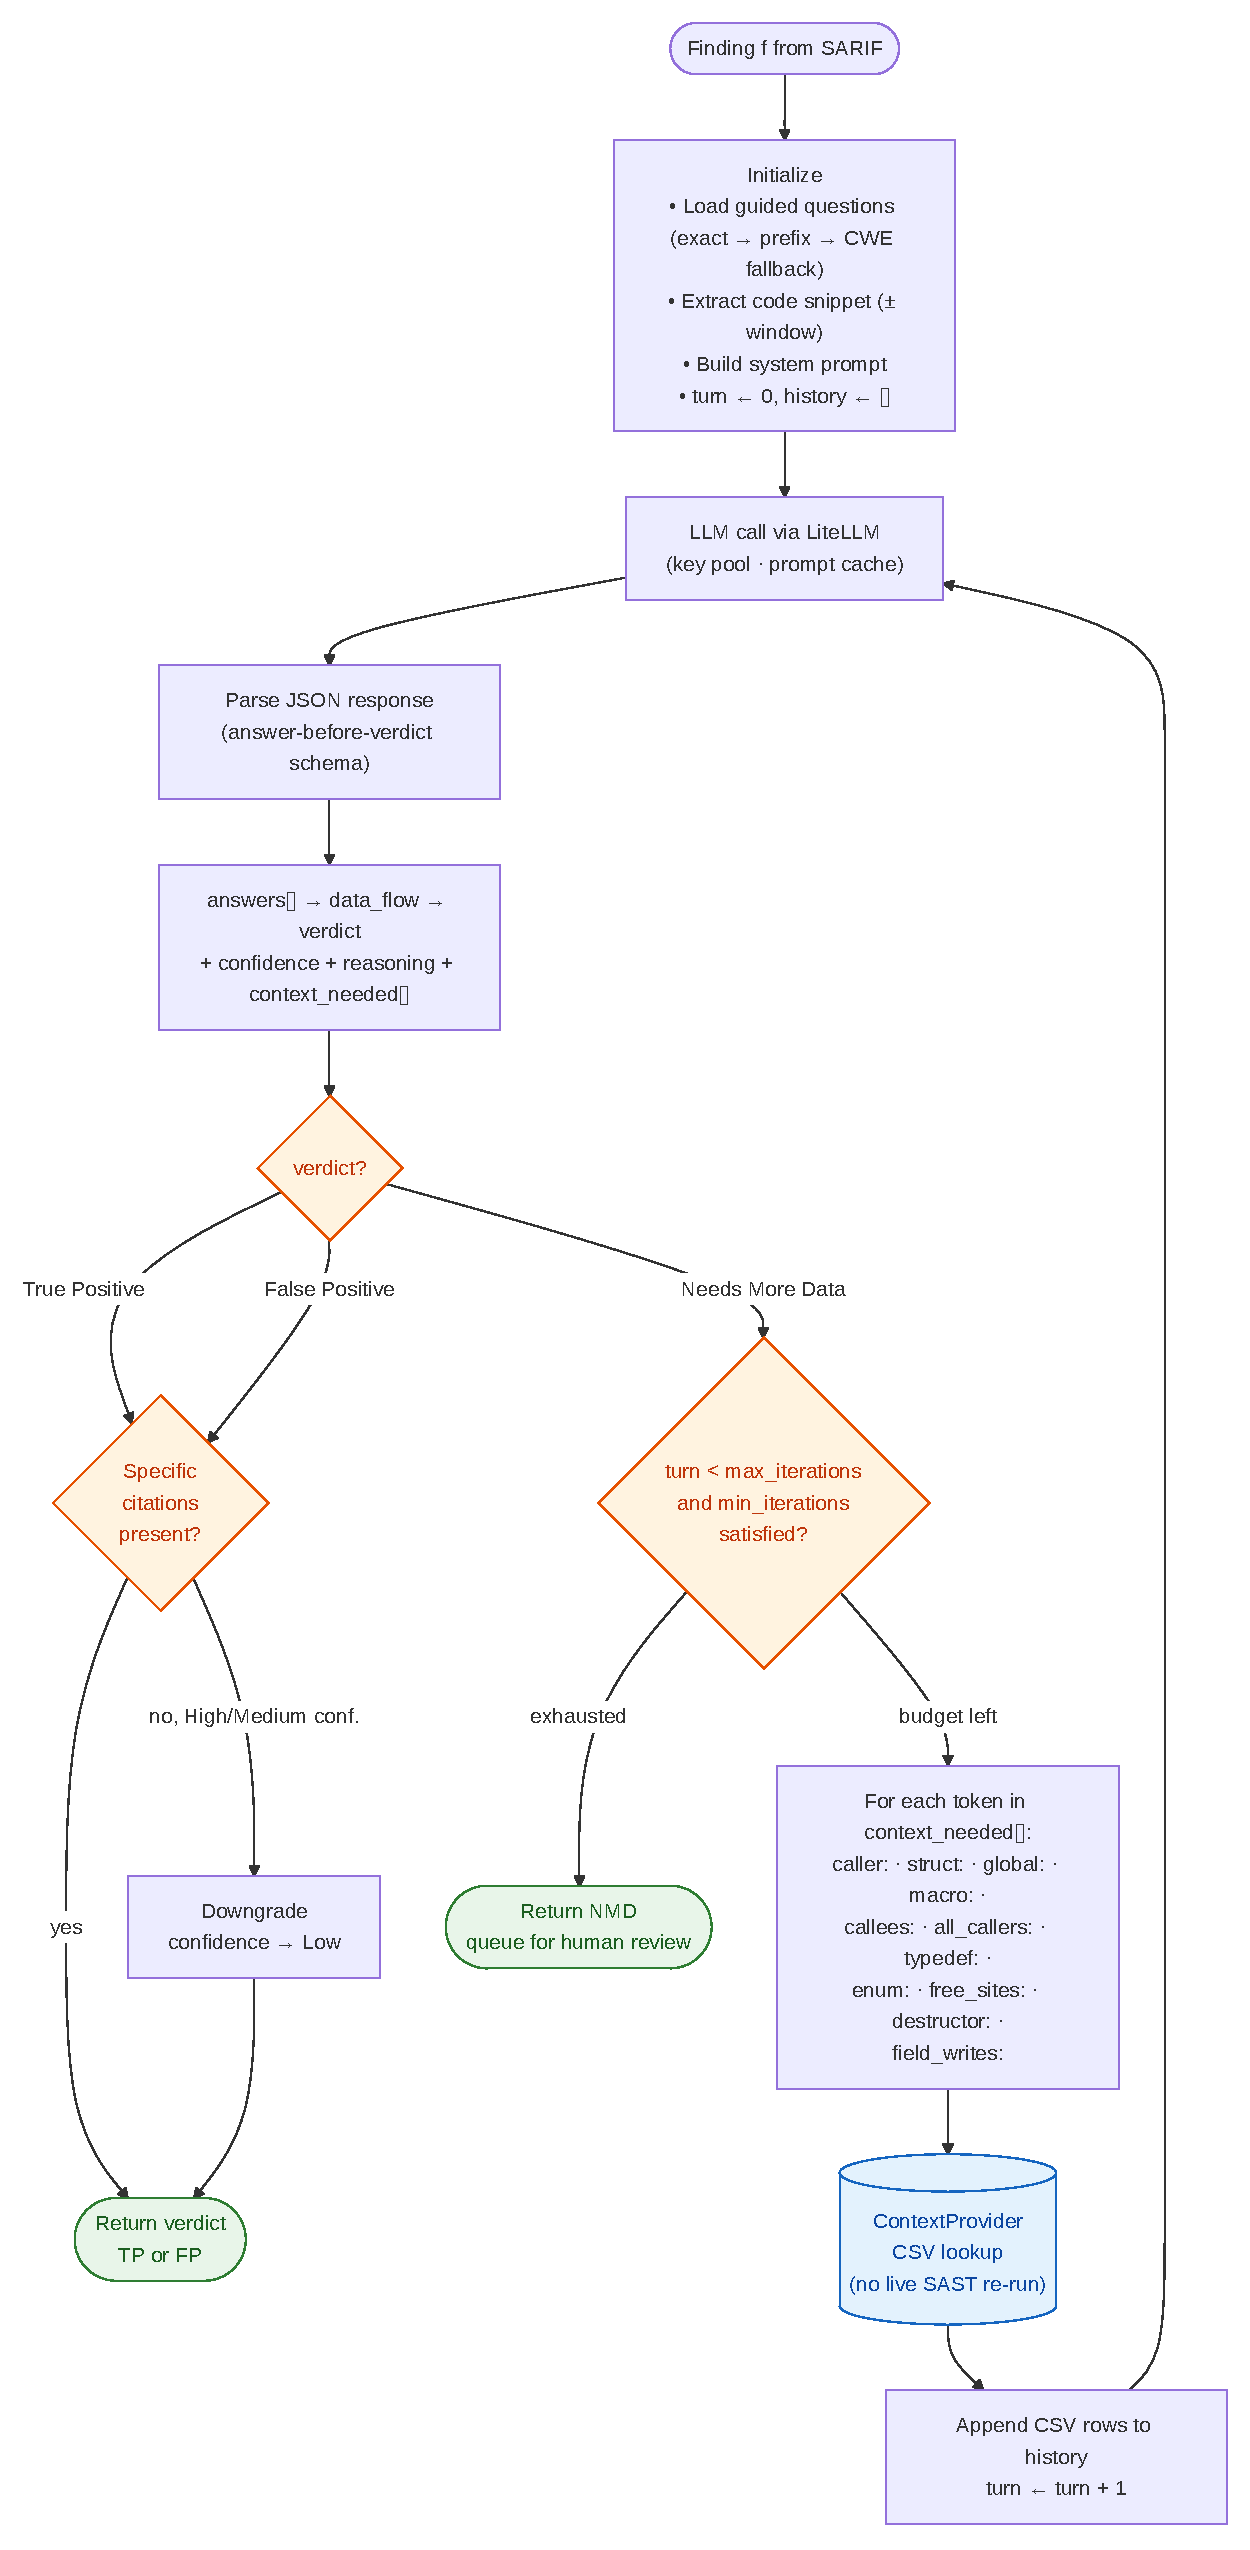
\includegraphics[width=\textwidth,height=0.70\textheight,keepaspectratio]{figures/verification.pdf}
  \caption{Per-finding LLM verification flow. The answer-before-verdict
  schema, the citation-based confidence downgrade, the fixed-vocabulary
  CSV broker, and the \texttt{min\_iterations} / \texttt{max\_iterations}
  loop guard. TP/FP terminate; NMD fetches additional context and
  re-enters the loop until budget exhaustion.}
  \label{fig:verification}
\end{figure}

\subsection{The context-request vocabulary}

The protocol defines a \textbf{fixed vocabulary} the LLM uses to
request context:

\begin{lstlisting}[language={}]
caller:<func>        struct:<type>          global:<var>
macro:<NAME>         callees:<func>         all_callers:<func>
typedef:<type>       enum:<name>            free_sites:<ptr>
destructor:<type>    field_writes:<T.f>
\end{lstlisting}

A constrained vocabulary is itself a hallucination control --- the LLM
cannot ask for \texttt{random\_thing:foo} and receive plausible-looking
nonsense; the provider returns nothing, and the LLM is forced to reason
with what it has or escalate.

\subsection{Tree-sitter fallback extractor}
\label{sec:treesitter}

The CSV broker described above is populated by stage 3, which by
default runs CodeQL queries against a per-repo CodeQL database. CodeQL
database creation, however, requires a working build for compiled
languages --- a hard precondition that fails routinely on closed-source
artifacts, deliberately opaque builds (Bazel/Buck without an
externalized dependency graph), and vendored or generated code paths.
A single such failure would otherwise disable the verifier on that
repository.

A \textbf{tree-sitter fallback extractor} at
\texttt{src/vuln\_hunter\_x/context/treesitter\_extractor.py} mitigates
this. When the CodeQL extraction path fails, the framework re-runs the
same per-language queries against a tree-sitter parse and emits CSVs
into the same schema the broker indexes, for: C, C++, Python,
JavaScript, Java, PHP, and Go (functions, callers, classes;
structs / globals / macros for C/C++). The cost is loss of
inter-procedural and type-resolution precision (tree-sitter sees
syntax, not semantics); the gain is that the context vocabulary
(\texttt{caller:} / \texttt{callees:} / \texttt{struct:} /
\texttt{typedef:} / \texttt{macro:}) stays answerable, so the
answer-before-verdict protocol degrades gracefully rather than
breaking.

The contract is isolated by interface: the LLM side is unchanged
regardless of which extractor produced the CSV row, so neither the
question banks nor the prompt template needs to know which backend was
in use. Tree-sitter precision should suffice for syntactic-class rules
(hard-coded credentials, unsanitized format strings, deprecated-API
uses); semantic-class rules (UAF, taint flows) continue to benefit
from a CodeQL backend when available.

% =====================================================================
\section{Tool- and Language-Agnostic Architecture}
\label{sec:architecture}

\subsection{SARIF as the only contract}
\label{sec:sarif-contract}

The framework treats SARIF as the \emph{only} contract between SAST
engines and the verification core. The \texttt{SarifParser} discovers
every \texttt{*.sarif} file under the repo's output directory; CodeQL,
Semgrep, and OpenGrep adapters write side-by-side SARIF and the
verifier processes the union, deduplicating by
\texttt{(rule\_id, file, line)}.

Adding a new SAST engine is a three-step contract:

\begin{enumerate}[leftmargin=*]
\item Implement an adapter that emits SARIF (most modern engines do
  natively).
\item Drop the SARIF into \texttt{output/<lang>/<repo>/}.
\item Optionally author rule-specific guided questions; otherwise the
  \texttt{default\_questions.yaml} fallback applies.
\end{enumerate}

No change to the verification engine, prompt, or context broker is
required. We have validated this contract for CodeQL 2.15+, Semgrep
1.x, and OpenGrep; we have draft adapters for SonarQube and Coverity.

\subsection{Developer-extensible custom signatures}
\label{sec:custom-signatures}

Triage is downstream of detection: an LLM verifier cannot recover from
a sink that no SAST rule fires on, however carefully it reasons. Real
defenders therefore need to \emph{extend} the detector --- to encode
the proprietary RPC frameworks, internal serialization formats, and
domain-specific dangerous APIs that vendor rule packs do not cover ---
and to have those extensions travel through the \emph{same}
verification protocol that built-in rules use. VulnHunterX implements
this through two parallel extension surfaces: a CodeQL surface for
queries with semantic taint or control-flow reasoning, and a
Semgrep / OpenGrep surface for syntactic pattern matching. Both are
authored locally, layered into a scan through a single profile flag,
and routed through the same rule-id matcher built-in rules use. The
current corpus:

\begin{table}[h]
\centering
\caption{Custom-signature corpus shipped with VulnHunterX.}
\label{tab:custom-corpus}
\small
\begin{tabular}{lrr}
\toprule
\textbf{Language} & \textbf{Custom CodeQL queries} & \textbf{Custom Semgrep/OpenGrep rules} \\
\midrule
C/C++       & 21 & 4  \\
Java        & 14 & 7  \\
JavaScript  & 15 & 9  \\
Python      & 12 & 12 \\
Go          & 11 & 8  \\
PHP         & ---  & 7  \\
\midrule
\textbf{Total} & \textbf{73} & \textbf{47} \\
\bottomrule
\end{tabular}
\end{table}

The remainder of this section specifies the authoring contract, the
layering mechanism, the routing path back to guided questions, the
audit tooling that holds the contract together, and a worked developer
workflow.

\subsubsection{Authoring contract}

Two contracts, one per engine.

\paragraph{CodeQL.} A custom query is a \texttt{.ql} file under
\texttt{config/codeql-custom/<lang>/src/}. The pack root carries a
\texttt{qlpack.yml} declaring a dependency on the appropriate
\texttt{codeql/<lang>-all} library, and a \texttt{suite.qls} that
enumerates the \texttt{.ql} files in \texttt{src/}. Each query declares:

\begin{lstlisting}[language={}]
@id          <lang>/<name>          // routes via tier-1 exact match
@kind        path-problem | problem // taint trace vs point finding
@tags        external/cwe/cwe-N security
@security-severity 5.0-9.0
\end{lstlisting}

The \texttt{@id} field is \textbf{load-bearing}: it lands verbatim in
the SARIF \texttt{ruleId}, which is the key the verifier matches
against the guided-question YAML. An \texttt{@id} of
\texttt{java/log4j-injection} routes immediately to a
\texttt{java/log4j-injection} entry in \texttt{java\_questions.yaml} if
one exists; otherwise the \texttt{@tags external/cwe/cwe-N} falls
through to the CWE tier
(Section~\ref{sec:routing}).

\paragraph{Semgrep / OpenGrep.} A custom rule is a YAML entry in
\texttt{config/semgrep-custom/<lang>.yaml}:

\begin{lstlisting}[language=yamlex]
- id: vulnhunterx.python.unsafe-yaml
  languages: [python]
  severity: ERROR
  metadata:
    cwe: ["CWE-502"]      # drives the CWE-question routing tier
    category: security
    owasp: "A08:2021"
  message: "Unsafe YAML load that allows arbitrary code execution"
  patterns:
    - pattern-either:
        - pattern: yaml.load(...)
        - pattern: yaml.full_load(...)
\end{lstlisting}

Semgrep IDs syntactically forbid the \texttt{/} character, so the
exact-match tier is structurally unavailable to Semgrep rules: every
custom Semgrep finding routes through the \textbf{CWE tier} instead.
The implication for the author is that \texttt{metadata.cwe} is not
optional and not cosmetic --- it is the \emph{only} channel through
which a custom Semgrep rule reaches a guided-question template; an
inaccurate or missing CWE silently demotes the rule to the default
question bank.

Both contracts are documented in
\texttt{config/codeql-custom/README.md} and
\texttt{config/semgrep-custom/README.md}.

\subsubsection{Profile-mediated layering}

Custom signatures are layered onto built-in suites by the \texttt{full}
profile in \texttt{config/rule\_categories.yaml} through two flags:

\begin{lstlisting}[language=yamlex]
full:
  include_custom_codeql: true
  custom_semgrep_path: "config/semgrep-custom/${LANG}.yaml"
\end{lstlisting}

At scan time the profile manager
(\texttt{RuleProfileManager.get\_codeql\_suites} in
\texttt{src/vuln\_hunter\_x/core/rule\_profiles.py}) appends
\texttt{config/codeql-custom/<codeql\_lang>/suite.qls} to the CodeQL
invocation as an extra suite; the CLI layer
(\texttt{src/vuln\_hunter\_x/cli/commands.py}, the analyze-command
handler) resolves the \verb|${LANG}| template against the repo's
language to produce the per-repo Semgrep config path, and skips empty
packs silently. The analyzer
(\texttt{run\_analysis(..., extra\_suites)} in
\texttt{src/vuln\_hunter\_x/codeql/analysis.py}) then invokes
\texttt{codeql database analyze <db> <builtin-suite> <extra-suite>} and
emits a single SARIF that the verifier consumes alongside the built-in
SARIF.

Authors who want to gate custom rules behind a non-default profile add
them to their fork's profile definition; \textbf{no engine code
changes} are required. The SARIF contract of
Section~\ref{sec:sarif-contract} that decouples engines also decouples
\emph{authors} from the verification core.

\subsubsection{Routing custom findings to guided questions}
\label{sec:routing}

The verifier's question loader
(\texttt{src/vuln\_hunter\_x/questions/loader.py},
\texttt{QuestionsLoader.get\_questions\_with\_match\_info}) tries six
match tiers in order:

\begin{enumerate}[leftmargin=*]
\item \textbf{exact} --- direct \texttt{ruleId} lookup against the
  per-language YAML key.
\item \textbf{normalized} --- hyphen $\leftrightarrow$ slash conversion.
\item \textbf{prefix} --- bidirectional prefix match.
\item \textbf{lang\_prefix} --- same-language rule-name match.
\item \textbf{cwe} --- CWE-id lookup via
  \texttt{cwe\_question\_map} in \texttt{config/rule\_categories.yaml}
  (100+ entries mapping CWE numbers to guided-question suffixes).
\item \textbf{default} --- fall through to
  \texttt{default\_questions.yaml}.
\end{enumerate}

A custom CodeQL query with \texttt{@id java/log4j-injection} hits
\textbf{tier 1} (exact match against the YAML key
\texttt{java/log4j-injection}). A custom Semgrep rule
\texttt{vulnhunterx.python.unsafe-yaml} with
\texttt{metadata.cwe: ["CWE-502"]} hits \textbf{tier 5}: the loader
maps \texttt{CWE-502 $\rightarrow$ "unsafe-deserialization"} and
resolves \texttt{py/unsafe-deserialization} against
\texttt{python\_questions.yaml}. Either path delivers the \emph{same}
guided-question + decision-rule template that built-in rules receive;
the only observable difference at the LLM end is the contents of the
\texttt{ruleId} field in the SARIF payload.

Extensibility along the SARIF contract is therefore both multi-engine
and multi-author: a defender-authored signature reaches the verifier
on the same path as a vendor-supplied built-in rule.

\subsubsection{Coverage audit tooling}

The four-step routing chain above --- custom-rule \texttt{@id} or
\texttt{metadata.cwe} $\rightarrow$ SARIF \texttt{ruleId}
$\rightarrow$ matcher tier $\rightarrow$ guided-question template ---
fails silently if any link breaks. Two failure modes recur in practice:
\textbf{rule rename}, where an engine upgrade renames a built-in rule
and the YAML still indexes the old id; and \textbf{CWE drift}, where a
newly-authored custom Semgrep rule declares a CWE that has no entry in
\texttt{cwe\_question\_map} and therefore routes to the default bank
without any visible error.

\texttt{scripts/audit\_rule\_coverage.py} cross-references every
guided-question YAML entry, every custom-rule \texttt{@id} and
\texttt{id}, and every \texttt{cwe\_question\_map} row, and emits three
artifacts under \texttt{output/audit/}:

\begin{itemize}[leftmargin=*]
\item \texttt{coverage\_matrix.csv} --- one row per
  \texttt{(lang, rule\_id)} with wiring flags for CWE-map presence and,
  with \texttt{--probe-tools}, for actual CodeQL / Semgrep emission
  against a probe sample.
\item \texttt{gap\_summary.md} --- gaps grouped by priority (A: rule
  has no route at all; B: rule routes only through a brittle prefix
  tier; C: cosmetically inconsistent).
\item \texttt{missing\_cwe\_map\_entries.yaml} --- a patch fragment a
  developer can paste into \texttt{config/rule\_categories.yaml} to
  close routing gaps in one motion.
\end{itemize}

The script exits with status 1 when any gap is detected, gating CI via
\texttt{--fail-on-gaps}; \texttt{--verify-packs} additionally confirms
that the Semgrep registry packs referenced by each profile still
resolve against the current registry index. The script is load-bearing
for the developer extensibility story: without it, custom rules
accumulate silently and the routing contract degrades in proportion to
the corpus's growth.

\subsubsection{Developer workflow (worked example)}

To make the contract concrete, consider a defender adding a Spring
Security misconfiguration query --- a finding that
\texttt{permitAll()} was applied to an endpoint covered by a sensitive
package prefix (CWE-285, improper authorization). The workflow:

\begin{enumerate}[leftmargin=*]
\item \textbf{Identify the sink and the CWE.}
  \texttt{HttpSecurity.authorizeRequests().permitAll()} reached from a
  config class touching a sensitive package. CWE-285.
\item \textbf{Write the CodeQL query.} Create
  \texttt{config/codeql-custom/java/src/spring-permitall.ql} declaring
  \texttt{@id java/spring-permitall},
  \texttt{@tags external/cwe/cwe-285 security}, and
  \texttt{@kind problem} or \texttt{@kind path-problem} depending on
  whether the analysis is point-level or taint-tracking.
\item \textbf{Author the guided-question template.} Add a
  \texttt{java/spring-permitall:} entry to
  \texttt{config/prompts/java\_questions.yaml} with anchored,
  evidence-binding questions (``anchor the \texttt{permitAll()}
  invocation line'', ``identify which URL pattern it applies to'',
  ``is there an overriding \texttt{authenticated()} call on a more
  specific pattern?'') and a closing decision rule (``only mark TP if
  the URL pattern resolves to a sensitive endpoint and no
  more-specific rule overrides it'').
\item \textbf{Run the scan.}
  \texttt{vuln-hunter-x analyze --tool codeql --profile full --local-path
  <repo> --lang java}. The \texttt{full} profile triggers the layering
  of the preceding subsection; the SARIF output carries the new
  \texttt{ruleId: java/spring-permitall}.
\item \textbf{Verify the routing.}
  \texttt{python scripts/audit\_rule\_coverage.py --probe-tools
  --fail-on-gaps}. A passing exit code confirms the \texttt{@id}
  matches a question template, the CWE map is intact, and the
  underlying CodeQL invocation actually emits the rule against a probe
  sample.
\item \textbf{Run verification.}
  \texttt{vuln-hunter-x verify --local-path <repo>}. The LLM receives
  the new guided-question template; verdicts emerge in the same JSON
  schema as built-in-rule verdicts.
\end{enumerate}

The walkthrough demonstrates that the protocol of
Sections~\ref{sec:questions}--\ref{sec:broker} applies \emph{unchanged}
to custom rules: the defender's threat model joins the
guided-question pipeline without any modification to the verifier, the
prompt template, or the context broker.

% ---- Pipeline figure (placed after § 6.2 to ground the developer flow) ----
\begin{figure}[t]
  \centering
  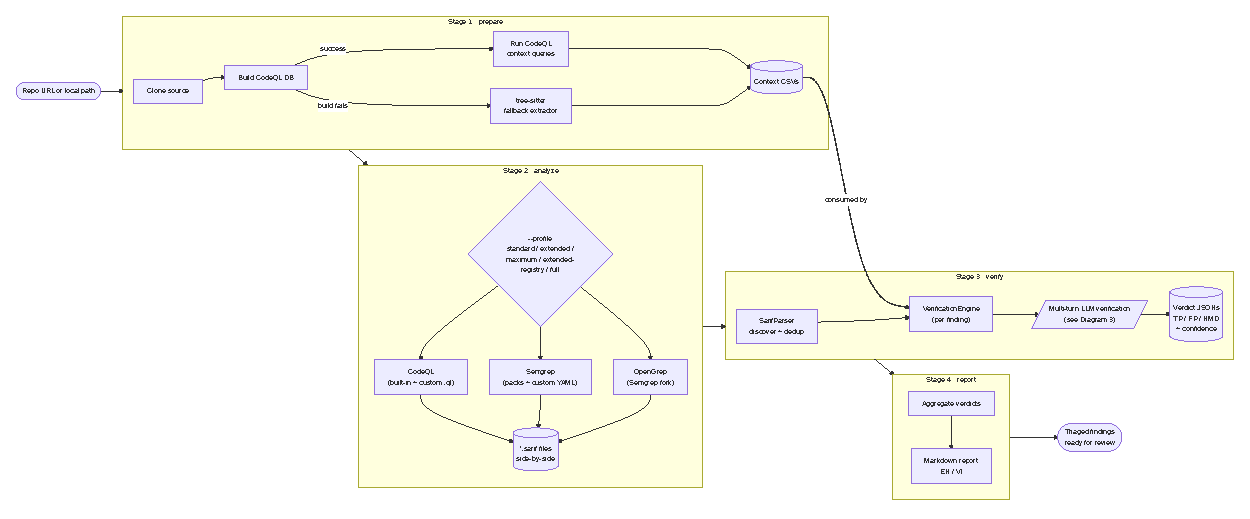
\includegraphics[width=\textwidth,height=0.45\textheight,keepaspectratio]{figures/pipeline.pdf}
  \caption{End-to-end pipeline (fuzzing stages excluded). Stage 1
  prepares the repository (clone, CodeQL DB, context CSVs with
  tree-sitter fallback); Stage 2 runs CodeQL / Semgrep / OpenGrep
  gated by a profile (\texttt{standard}, \texttt{extended},
  \texttt{maximum}, \texttt{extended-registry}, \texttt{full}) that
  controls custom-rule layering; Stage 3 dispatches each SARIF finding
  through the multi-turn LLM verifier of
  Figure~\ref{fig:verification}; Stage 4 aggregates verdicts into a
  markdown report.}
  \label{fig:pipeline}
\end{figure}

\subsection{Rule profiles}

Five named profiles, defined in \texttt{config/rule\_categories.yaml},
gate the SAST scan-time configuration:

\begin{table}[h]
\centering
\caption{Rule-profile coverage matrix.}
\label{tab:profiles}
\footnotesize
\begin{tabularx}{\textwidth}{@{}llXX@{}}
\toprule
\textbf{Profile} & \textbf{CodeQL suite} & \textbf{Semgrep packs} & \textbf{Custom rules} \\
\midrule
\texttt{standard} (default) & security-extended    & \texttt{auto} & --- \\
\texttt{extended}           & security-extended    & + \texttt{p/security-audit}, \texttt{p/secrets} & --- \\
\texttt{maximum}            & security-and-quality & + \texttt{p/owasp-top-ten} & --- \\
\texttt{extended-registry}  & security-and-quality & 8 universal + per-language packs & --- \\
\texttt{full}               & security-and-quality & extended-registry packs & + \texttt{config/codeql-custom/} + \texttt{config/semgrep-custom/} \\
\bottomrule
\end{tabularx}
\end{table}

A \texttt{language\_specific\_configs} field lets per-language packs
be added without polluting other-language scans (e.g.~\texttt{p/django}
only applied to Python repos). The profile is a knob along the
\emph{coverage} $\times$ \emph{cost} $\times$ \emph{latency} axis:
inline-CI use favours \texttt{standard} and \verb|--max-iterations 1|
(zero-shot CoT, ZeroFalse-style); nightly or on-merge audit favours
\texttt{full} with the multi-turn protocol. Profile choice is
orthogonal to the verification protocol ---
Sections~\ref{sec:questions}--\ref{sec:broker} apply unchanged
regardless.

\subsection{Language-uniform static verification, multi-language dynamic stages}

Static verification, the subject of this paper, is
\textbf{language-uniform}: the guided-question YAML \emph{is} the
language adapter, and Sections~\ref{sec:questions}--\ref{sec:broker}
contain no per-language code paths beyond the YAML registry.
Dynamic-testing stages 5--8 are by necessity per-language and use the
\texttt{LanguageBackend} abstraction with backends for C/C++
(libFuzzer / sanitizers), Python (Atheris), Java (Jazzer), JavaScript
(Jazzer.js), and PHP (php-fuzzer). These stages are \emph{complementary
downstream} validation --- they attempt to reproduce a TP verdict as a
runtime crash --- and are out of scope for this paper.

% =====================================================================
\section{Threats to Validity}
\label{sec:threats}

We consolidate the threats to validity into a single section structured
around the standard four-class taxonomy (Wohlin et al., 2012),
reframed for a methodological contribution: the threats here apply to
the \emph{transferability} and \emph{interpretability} of the
methodology, with comparative-empirical threats deferred to the
companion evaluation paper.

\subsection{Construct validity}

The construct \textbf{``guided question''} is operationalized by the
three properties (P1) evidence-binding, (P2) atomicity, (P3) refusal-
admissibility in Section~\ref{sec:questions}.1. Question authorship can
violate these properties silently --- e.g., a compound question that
bundles two sub-facts will pass YAML loading but degrade
evidence-binding. We mitigate with author discipline (the five-step
procedure of Section~\ref{sec:question-authoring}) and the coverage
audit (Section~\ref{sec:audit}); we acknowledge that no automated
check enforces P1--P3 against the \emph{content} of a question, only
the \emph{presence} of an entry.

A secondary construct concern is \textbf{ground-truth labelling} in
any downstream empirical evaluation: CVE-linked patches encode patch
equivalence, not always semantic equivalence, and the labelled-function
boundary may differ from the precise vulnerable statement. This is a
threat to the companion empirical paper rather than to the methodology
specified here.

\subsection{Internal validity}

The methodology bundles three contributions --- guided questions
(Section~\ref{sec:questions}), answer-before-verdict schema
(Section~\ref{sec:protocol}), and multi-turn context brokering
(Section~\ref{sec:broker}) --- and uses them together. The paper does
\textbf{not} empirically isolate the contribution of each.
Schema-reordering and generic-vs-specialised-question ablations are
planned in the companion empirical paper; without them, the
methodology is internally consistent but its component contributions
are not individually attributable from the present work.

\subsection{External validity}
\label{sec:external-validity}

A second external threat is \textbf{single-author corpus bias}: the
342 guided-question templates were authored by one analyst. Triage
style may encode author-specific heuristics that do not transfer.
Inter-rater consistency studies are queued. The rule-coverage audit
(Section~\ref{sec:audit}) surfaces \emph{coverage} gaps but not
\emph{quality} gaps --- that requires a second author.

The custom-signature corpus (73 CodeQL + 47 Semgrep / OpenGrep) is
similarly authored, and its language distribution is uneven (no PHP
custom CodeQL queries; C/C++ Semgrep coverage is thin at four rules).
Defenders adopting the framework should expect to \emph{extend} the
corpus, not adopt it verbatim.

A third external threat is the \textbf{architecture-blindness} of the
scanner layer: language-specific rule packs are applied uniformly
without inferring the runtime framework from manifest files. We
discuss this in Section~\ref{sec:eng-limits} and record it in
Appendix~\ref{sec:tov-checklist} as the highest-priority piece of open
engineering work.

\subsection{Conclusion validity}

This paper makes \textbf{no quantitative claims} (precision, recall,
F1, cost). It therefore makes no significance-testing claims. The
companion empirical paper reports Wilson confidence intervals,
McNemar's test for paired comparison against raw-SAST, and bootstrap
confidence intervals on F1, on three datasets (Juliet C/C++, OWASP
Benchmark Java, CASTLE).

\subsection{Ethical validity and responsible use}

VulnHunterX is a defensive tool: it triages already-flagged alerts in
the defender's own codebase. It does not perform vulnerability
discovery in third-party software, does not generate exploits, and
does not handle unauthorized targets. The dynamic-testing stages 6--8
(libFuzzer / Atheris / Jazzer harnesses) are likewise defensive and
require local source access. We urge users to obtain authorization
before running the framework on any codebase they do not own.

The framework's reliance on commercial LLM APIs raises a \emph{data
exfiltration} concern when source code is shipped to a third-party
model. We mitigate with first-class support for local inference
(Ollama) and with the CSV broker, which transmits only minimal slices
rather than whole repositories.

% =====================================================================
\section{Discussion}
\label{sec:discussion}

\subsection{Why cheap LLMs may work here}

Conventional wisdom, supported by SecLLMHolmes' $\approx$40\% accuracy
figures for frontier models, treats security reasoning as the domain
in which model size matters most. A refinement is plausible here:
\textbf{size matters when the model is asked to make a judgment; when
the model is asked to extract evidence and apply a fixed decision
rule, much smaller models may suffice.} The guided-question protocol
offloads \emph{judgment} to the rule author (who fixes the decision
rule) and leaves only \emph{evidence extraction} and \emph{rule
application} to the LLM, both more tractable for smaller models. This
is a hypothesis, not a finding established here; the model-size sweep
in the companion evaluation paper is its empirical test.

\subsection{Relationship to retrieval-augmented generation}

The context broker (Section~\ref{sec:broker}) is a constrained form
of retrieval-augmented generation (RAG) in which the \emph{retrieval
vocabulary} is fixed by the protocol designer rather than learned.
The trade-off is expressivity for safety: the LLM cannot ask
arbitrary questions of the codebase, but it also cannot receive
plausible-looking nonsense. Constrained-vocabulary RAG suits
high-assurance domains for the same reason. The tree-sitter fallback
(Section~\ref{sec:treesitter}) reinforces the point: the retrieval
\emph{interface} is preserved across two structurally different
extraction backends precisely because the vocabulary is fixed, not
learned.

\subsection{Engineering limitations}
\label{sec:eng-limits}

Three engineering limitations are worth flagging beyond the
methodological threats catalogued in Section~\ref{sec:threats}:

\begin{itemize}[leftmargin=*]
\item \textbf{Question authorship cost.} Each new rule benefits from a
  hand-authored question set; full coverage of CodeQL's 1{,}000+ rules
  is an open project. A default fallback
  (Section~\ref{sec:questions}.5) and the coverage audit
  (Section~\ref{sec:audit}) at least \emph{surface} the gap inventory;
  the \emph{upper bound} on what specialization buys is left to an
  ablation in the companion paper.

\item \textbf{Context completeness.} The CSV broker is bounded by what
  was extracted in stage 3 (\texttt{extract-context}); the tree-sitter
  fallback (Section~\ref{sec:treesitter}) covers the
  CodeQL-DB-build-failure threat, but inter-procedural reasoning
  across repository or library boundaries --- e.g.~into vendored
  libraries or generated code outside the extracted per-symbol tables
  --- remains a gap.

\item \textbf{Application-architecture blindness.} VulnHunterX is
  language-aware but \textbf{architecture-blind}: it does not infer a
  repository's framework or runtime from manifest files
  (\texttt{package.json}, \texttt{requirements.txt},
  \texttt{composer.json}, \texttt{pom.xml}, \texttt{go.mod}) and does
  not route scans by detected framework. The \texttt{full} profile
  applies framework-specific Semgrep packs (\texttt{p/django},
  \texttt{p/flask}, \texttt{p/nodejs},
  \texttt{p/eslint-plugin-security}) uniformly across every repository
  of the matching language, and custom Semgrep rules that
  pattern-match framework idioms (e.g., \verb|req.body.$X| for
  Express, \verb|$APP.run(..., debug=True)| for Flask) silently fail
  on non-matching runtimes. This produces two failure modes
  symmetrically: (i) \textbf{false positives} when a Django- or
  Express-flavoured rule fires on a CLI tool that imports the package
  for code reuse but never serves a request; (ii) \textbf{false
  negatives} when a service's actual sinks have no rule because all
  ``web'' rules assumed an Express or Flask handler. Context CSVs
  (functions, callers, classes) are AST-level and carry no framework
  annotation, so the LLM verifier cannot recover the lost
  architectural signal from context alone. Existing mitigations are
  partial: the guided questions include conditional branches (``If
  using Sequelize\ldots'', ``If using React's
  \texttt{dangerouslySetInnerHTML}\ldots'') but these enumerate
  possibilities rather than route by detected framework, and
  \texttt{min\_iterations $\geq$ 2} is enforced on taint-CWE findings
  for Python / JavaScript / Java / PHP / Go as a pragmatic workaround.
  A principled fix --- manifest-driven framework detection that gates
  rule packs at scan time and annotates context CSVs with framework
  tags consumable by the guided-question matcher --- is the
  highest-priority piece of open engineering work and is recorded as
  such in Appendix~\ref{sec:tov-checklist}.
\end{itemize}

% =====================================================================
\section{Reproducibility and Artifact}
\label{sec:repro}

The framework, all six guided-question corpora, the custom CodeQL and
Semgrep rule packs, the rule-coverage audit script
(\texttt{scripts/audit\_rule\_coverage.py}), the tree-sitter context
fallback
(\texttt{src/vuln\_hunter\_x/context/treesitter\_extractor.py}), and
the benchmark harness are released under the MIT license. Installation
and a one-finding sanity run:

\begin{lstlisting}[language=bashex]
git clone <repo> && cd VulnHunterX
uv venv --python python3.12 .venv && source .venv/bin/activate
pip install -e ".[dev]"
vuln-hunter-x check-env

# Triage a single repo (CodeQL + Semgrep + OpenGrep, full profile):
vuln-hunter-x prepare --local-path /path/to/repo --lang <lang>
vuln-hunter-x analyze --tool all --profile full \
                      --local-path /path/to/repo --lang <lang>
vuln-hunter-x verify  --local-path /path/to/repo
\end{lstlisting}

Long-running evaluations use the resumable benchmark harness:

\begin{lstlisting}[language=bashex]
python benchmarks/scripts/run_benchmark.py \
    --run-dir benchmarks/results/my_run \
    --dataset juliet --approach vulnhunterx \
    --model <provider/model-id>

# Resume from the last checkpoint after interruption:
python benchmarks/scripts/run_benchmark.py \
    --run-dir benchmarks/results/my_run --resume

# Re-execute only entries that previously errored (one entry-id per line):
python benchmarks/scripts/run_benchmark.py \
    --run-dir benchmarks/results/my_run \
    --only-entries failed_entries.txt
\end{lstlisting}

Authoring a new custom signature follows the contract of
Section~\ref{sec:custom-signatures}; the routing wiring is validated
in CI by:

\begin{lstlisting}[language=bashex]
python scripts/audit_rule_coverage.py --probe-tools --fail-on-gaps
\end{lstlisting}

% =====================================================================
\section{Conclusion}
\label{sec:conclusion}

The cost-vs-accuracy frontier of LLM-based SAST triage is plausibly
moved by \textbf{reasoning structure}, not model size. VulnHunterX
combines per-rule guided questions, answer-before-verdict at the
schema level, a fixed-vocabulary context broker with a seven-language
tree-sitter fallback, and a single profile flag through which defenders
layer their own CodeQL queries and Semgrep / OpenGrep rules onto
built-in suites. The result is a six-language triage layer in which
the guided-question methodology lives as a deployable, extensible
artifact. Three open questions remain:

\begin{itemize}[leftmargin=*]
\item \textbf{Empirical attribution.} Which methodological lever ---
  guided questions, answer-before-verdict schema, or multi-turn
  context brokering --- contributes most to precision and recall? The
  companion evaluation paper on Juliet C/C++, OWASP Benchmark (Java),
  and CASTLE will isolate these via schema-reordering,
  generic-vs-specialised-question, and
  single-turn-vs-multi-turn ablations.
\item \textbf{Application-architecture blindness.} Closing the
  framework-detection gap (Section~\ref{sec:eng-limits}) ---
  manifest-driven runtime inference that gates rule packs at scan time
  and annotates context CSVs with framework tags --- is the
  highest-priority open engineering work.
\item \textbf{Inter-rater corpus stability.} All 342 guided-question
  templates were authored by a single analyst; inter-rater consistency
  studies are needed to quantify single-author style bias.
\end{itemize}

We release the framework, the six-language guided-question corpora
(342 templates, 4{,}676 lines), the 73 custom CodeQL queries and 47
custom Semgrep / OpenGrep rules, the rule-coverage audit script, and
the benchmark harness under MIT to support community extension.

% =====================================================================
\appendix

\section{Example Guided Question Set}
\label{app:question-example}

From \texttt{config/prompts/cpp\_questions.yaml}
(\texttt{cpp/use-after-free}, abridged):

\begin{lstlisting}[language=yamlex]
cpp/use-after-free:
  short_description: "Use of pointer after memory has been freed"
  questions:
    - "ANCHOR FIRST: quote the EXACT statement at the flagged line ..."
    - "If the snippet contains MULTIPLE functions ..."
    - "Where is the pointer at the flagged line ALLOCATED ..."
    - "List ALL free()/delete calls reachable from the flagged use ..."
    - "Is the pointer set to NULL immediately after EACH free? ..."
    - "For EACH (free_site, flagged_use) pair: describe the SHORTEST ..."
    - "Does the pointer escape this function ..."
    - "Are there ALIAS pointers ..."
    - "If the pointer is REASSIGNED between free and use ..."
    - "DECISION RULE: only mark TP if you can produce a SPECIFIC triple ..."
  additional_context: ["caller", "struct", "callees", "all_callers",
                       "free_sites", "destructor", "field_writes"]
  min_iterations: 2
  snippet_window_lines: 60
\end{lstlisting}

\section{Context-Request Grammar (BNF)}
\label{app:bnf}

\begin{lstlisting}[language={}]
request    ::= verb ":" arg
verb       ::= "caller"   | "struct"     | "global"
             | "macro"    | "callees"    | "all_callers"
             | "typedef"  | "enum"       | "free_sites"
             | "destructor" | "field_writes"
arg        ::= identifier ("." identifier)?
\end{lstlisting}

\section{Threats-to-Validity Checklist}
\label{sec:tov-checklist}

\begin{longtable}{@{}p{0.10\textwidth} p{0.36\textwidth} p{0.46\textwidth}@{}}
\toprule
\textbf{Class} & \textbf{Threat} & \textbf{Mitigation} \\
\midrule
\endhead
Construct &
Question authorship may silently violate P1--P3 &
Five-step authoring procedure
(Section~\ref{sec:question-authoring}); audit script for coverage
(Section~\ref{sec:audit}); content quality requires second author \\
\addlinespace
Construct &
Ground-truth label disputes in any downstream eval &
CVE-patch linkage with manual spot-check; reserved for companion
empirical paper \\
\addlinespace
Internal &
Per-component contribution not isolated &
Planned schema-reordering and generic-vs-specialised ablations in
companion empirical paper \\
\addlinespace
External &
Single-author question-bank style bias &
Inter-rater study queued
(Section~\ref{sec:external-validity}); audit script surfaces gap
inventory (Section~\ref{sec:audit}) \\
\addlinespace
External &
Uneven custom-signature corpus across languages &
Defenders should extend, not adopt verbatim; authoring contract
documented (Section~\ref{sec:custom-signatures}) \\
\addlinespace
External &
\textbf{Architecture-blind scanning} produces both FPs
(irrelevant framework rules firing on non-framework code) and FNs
(framework idioms unmatched on differently-framed services) &
Conditional guided-question branches; forced 2-iteration verification
on taint CWEs for framework languages; manifest-driven framework
detection is open work (Section~\ref{sec:eng-limits}) \\
\addlinespace
Conclusion &
No quantitative claims to test &
Paper makes no significance claims; companion eval reports Wilson CIs,
McNemar, bootstrap CIs \\
\addlinespace
Ethical &
Source exfiltration to LLM APIs &
Local-inference support (Ollama); CSV slicing; tree-sitter fallback
(Section~\ref{sec:treesitter}) avoids shipping uncompiled code through
CodeQL DB \\
\addlinespace
Engineering &
CodeQL DB build required for context extraction &
Tree-sitter fallback (Section~\ref{sec:treesitter}) covers 7 languages
with same CSV schema \\
\bottomrule
\end{longtable}

% =====================================================================
\begin{thebibliography}{99}

\bibitem{avgustinov2016ql}
P.~Avgustinov et al. (2016).
\newblock QL: Object-Oriented Queries on Relational Data.
\newblock \emph{SLE 2016}.

\bibitem{christakis2016developers}
M.~Christakis and C.~Bird (2016).
\newblock What developers want and need from program analysis: an
  empirical study.
\newblock \emph{ASE 2016}.

\bibitem{cousot1977abstract}
P.~Cousot and R.~Cousot (1977).
\newblock Abstract interpretation.
\newblock \emph{POPL 1977}.

\bibitem{hanam2014patterns}
Q.~Hanam et al. (2014).
\newblock Finding patterns in static analysis alerts.
\newblock \emph{MSR 2014}.

\bibitem{heckman2011actionable}
S.~Heckman and L.~Williams (2011).
\newblock A systematic literature review of actionable alert
  identification techniques.
\newblock \emph{Information and Software Technology 53(4)}.

\bibitem{imtiaz2019composition}
N.~Imtiaz et al. (2019).
\newblock A comparative study of vulnerability reporting by software
  composition analysis tools.
\newblock \emph{ESEM 2019}.

\bibitem{johnson2013why}
B.~Johnson et al. (2013).
\newblock Why don't software developers use static analysis tools?
\newblock \emph{FSE 2013}.

\bibitem{yoon2014active}
J.~Yoon et al. (2014).
\newblock Reducing false alarms via active learning.
\newblock \emph{ASE 2014}.

\bibitem{su2024llm4fpm}
F.~Su et al. (2024).
\newblock LLM4FPM: Utilizing Precise and Complete Code Context to
  Guide LLM in Automatic False Positive Mitigation.
\newblock \href{https://arxiv.org/abs/2411.03079}{arXiv:2411.03079}.

\bibitem{mohajer2025zerofalse}
M.~M.~Mohajer et al. (2025).
\newblock ZeroFalse: Improving Precision in Static Analysis with LLMs.
\newblock \href{https://arxiv.org/abs/2510.02534}{arXiv:2510.02534}.

\bibitem{ullah2024secllmholmes}
S.~Ullah, M.~Han et al. (2024).
\newblock LLMs Cannot Reliably Identify and Reason About Security
  Vulnerabilities in Code.
\newblock \href{https://arxiv.org/abs/2312.12575}{arXiv:2312.12575},
  \emph{IEEE S\&P 2024}.

\bibitem{risse2025llmxcpg}
N.~Risse et al. (2025).
\newblock LLMxCPG: Code Property Graph-Guided LLM for Vulnerability
  Detection.
\newblock \href{https://arxiv.org/abs/2507.16585}{arXiv:2507.16585},
  \emph{USENIX Security 2025}.

\bibitem{bouzenia2025castle}
M.~Bouzenia et al. (2025).
\newblock CASTLE: Benchmarking Dataset for Static Code Analyzers and
  LLMs towards CWE Detection.
\newblock \href{https://arxiv.org/abs/2503.09433}{arXiv:2503.09433},
  \emph{TASE 2025}.

\bibitem{li2025cisc}
B.~Li et al. (2025).
\newblock CISC: Self-Consistency with Confidence for LLM-Based Code
  Review.
\newblock \emph{ACL 2025 Findings}, paper 1030.

\bibitem{croft2023empirical}
R.~Croft et al. (2023).
\newblock An Empirical Study of Deep Learning Models for Vulnerability
  Detection.
\newblock \emph{ICSE 2023}.

\bibitem{chen2023diversevul}
Y.~Chen et al. (2023).
\newblock DiverseVul: A New Vulnerable Source Code Dataset for Deep
  Learning Based Vulnerability Detection.
\newblock \emph{RAID 2023}.

\bibitem{wohlin2012experimentation}
C.~Wohlin et al. (2012).
\newblock \emph{Experimentation in Software Engineering}.
\newblock Springer.

\bibitem{oasis2020sarif}
OASIS (2020).
\newblock SARIF Version 2.1.0.

\end{thebibliography}

\end{document}
